\section{\name Overview} \label{sec:overview}
\yueqiang{
requirements:
1) minimum modifications (SLoC);
2) keeping security (we need a short subsection to discuss the security)
3) minimum effects on page table allocation/deallocation in terms of memeory and CPU usage
}
\yueqiang{
algorithm: life cycle of pt cache (allocation, free)
pt cache(mechanism) enable and disable
}
%overview
Before we illustrate the design rationale of \name, we first describe the desired requirements that \name meets as follows:

R1) Retaining security. \name aims at reducing IOTLB flush while guaranteeing existing security strength.
R2) Achieving as good as possible performance. While benefitting IOTLB performance, \name is supposed to achieve positive results in the aspects of CPU and memory usage.
R3) Slightest possible modifications to Xen and Linux kernel for the sake of compatibility.

\subsection{Design Rationale}
\name enforces access control at a finer granularity to protect guest page tables without flushing IOTLB. Besides, guest OS builds up cache pools to manage these pages to facilitate the speed of page table allocation/deallocation, gaining big benefits of CPU efficiency while causing small impacts on memory usage.

\subsubsection{Access Control at A Finer Granularity}
%firstly, talk about how to reduce the IOTLB flush.
As revealed in previous sections, for writable pages, Xen allows write-access both for guest OS and assigned I/O devices. However, \name performs DMA prevention for specified writable pages. If they are updated to be of page-table type, Xen only limits OS to read-only permission without affecting I/O page tables as well as IOTLB, still defending attacks from both sides.

Specifically, Xen maintains a new flag bit called \textbf{cache} with a machine page, indicating that the corresponding page is free from DMA-access. Whatever page type a machine page is, if it is determined to own the flag, Xen neither maps nor unmaps the page from I/O page tables, thus avoiding an IOTLB-flush. As only page type updates between writable and page-table are considered, the cache flag is along with the two types. If guest OS creates a new page-table, Xen firstly reuses the validation process to enforce software protection, and then checks if the specific page has the safe flag. If not, Xen sets the page with the new flag and enforces DMA protection. If so, Xen has nothing to do but updates the page to be a safe page-table. As for the guest page table destruction, Xen also reuses existing operations to remove software protection, after which each page is set with the safe flag and updated to be writable while DMA protection is still maintained. In this way, every time a process is created/destructed, corresponding pages will own the safe flag, indicating that they are under DMA protection. Figure \ref{fig:safe-flag} describes how WR-inter-PT varies with the flag.

Therefore, when validating a writable page with the ready flag (a safe writable page) to be of page-table, Xen only needs to revoke write-permission from the OS without unmapping the page from I/O page tables, avoiding an expensive IOTLB-flush. Also, \name proposes a novel cache algorithm in the guest OS to manage safe writable pages in order to prevent unacceptable exceptions caused by devices and facilitate the speed of creating/destructing page tables.
Ensuring security is demonstrated below.

\begin{figure}[ht]
\centering
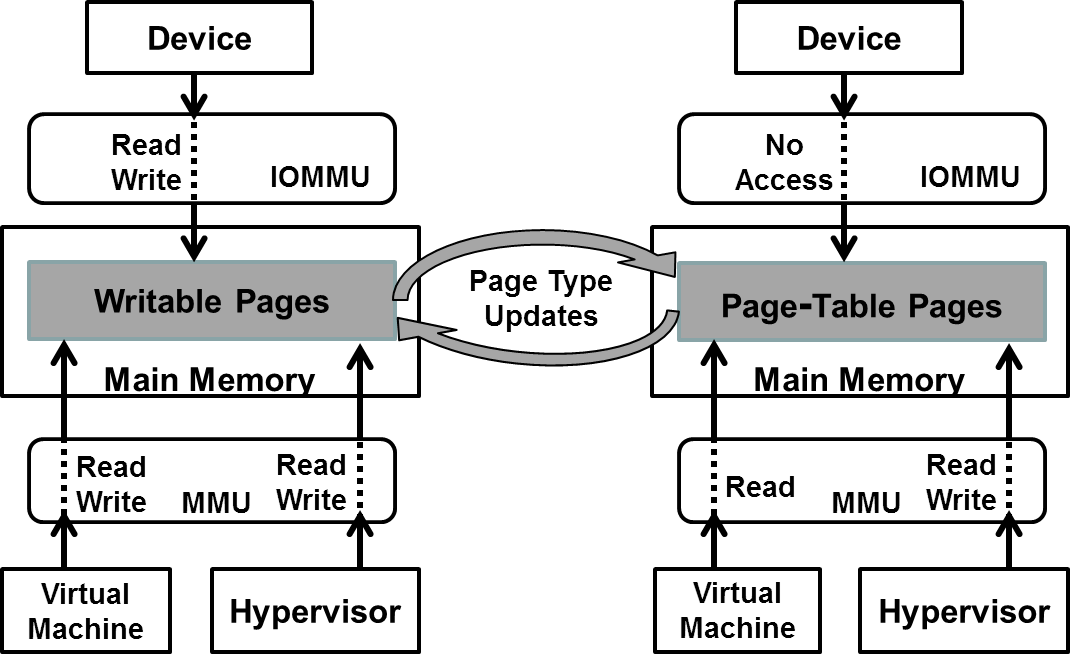
\includegraphics[width=0.5\textwidth]{image/background/wr2pt.png} \\
\caption{Page Type Updates With Safe Flag}
\label{fig:safe-flag}
\end{figure}

\subsection{Cache Algorithm}
%secondly, design the cache pool to support it



enforce security polices in two aspects, i.e., guest OS and assigned I/O devices.Because of that, we associates the ready flag with

writable pages are writable for both guest OS and assigned I/O devices while

, , and  We defines that a writable page with a flag called \textbf{ready} that can be write-accessed by OS while inaccessible to devices. Because of that, when OS writes its writable pages with the ready flag (ready writable pages) as new page tables and submits the request of updating page tables, Xen reuses the existing validation process, however will not have to unmap them from I/O page tables instead the \textbf{ready} flag is marked with the page-table pages (ready page-table pages), thus reducing IOTLB-flushes. Besides, since the definition of page type is transparent to the OS, it needs to build a cache pool especially for the ready writable pages rather than free them into the buddy system which reserves only writable pages. Also, this cache mechanism benefits time efficiency when.

while provides every level of page-table cache pool for guest OS
